\documentclass{article}

    \usepackage{fancyhdr}
    \usepackage{extramarks}
    \usepackage{amsmath}
    \usepackage{amsthm}
    \usepackage{amsfonts}
    \usepackage{tikz}
    \usepackage{amssymb}
    \usepackage{subcaption}
    \usepackage{blkarray}
    \usetikzlibrary{arrows, automata}
    \usepackage{forest}
    \usetikzlibrary{chains,positioning} %

    \usepackage{algorithm}
    \usepackage{algorithmicx}

    \usepackage{mathtools}
    \usepackage{bm}
    \usepackage{esvect}


    

    \makeatletter
    \def\BState{\State\hskip-\ALG@thistlm}
    \makeatother


    \newcommand{\Mod}[1]{\ (\mathrm{mod}\ #1)}

    


    \usepackage{enumitem}

    \setlist[enumerate,1]{start=0} % only outer nesting level


    \usepackage{tabulary}

\usepackage[newcommands]{ragged2e}

    \usetikzlibrary{trees}

    \newcommand{\question}{\textbf{Question:}}
    \newcommand{\answer}{\textbf{Answer:}}
    \newcommand{\modx}{\;(\bmod\;}

    


    \usetikzlibrary{decorations.markings}
    \tikzstyle{vertex}=[circle, draw, inner sep=0pt, minimum size=6pt]
    \newcommand{\vertex}{\node[vertex]}

    
    \usepackage{amsmath}
    \usepackage{algorithm}
    \usepackage[noend]{algpseudocode}
    \usepackage[utf8]{inputenc}
    \usepackage{enumerate}
    \usepackage{geometry}
    \usepackage{mathtools}
    \usepackage{parskip}
    \usepackage{xifthen, xparse}
    
    \algdef{SE}[SUBALG]{Indent}{EndIndent}{}{\algorithmicend\ }%
    \algtext*{Indent}
    \algtext*{EndIndent}
    
    
    
    \usetikzlibrary{automata,positioning}
    
    %
    % Basic Document Settings
    %
    
    \topmargin=-0.45in
    \evensidemargin=0in
    \oddsidemargin=0in
    \textwidth=6.5in
    \textheight=9.0in
    \headsep=0.25in
    
    \linespread{1.1}
    
    \pagestyle{fancy}
    \lhead{\hmwkAuthorName}
    \chead{\hmwkClass\ \hmwkTitle}
    \rhead{\firstxmark}
    \lfoot{\lastxmark}
    \cfoot{\thepage}
    
    \renewcommand\headrulewidth{0.4pt}
    \renewcommand\footrulewidth{0.4pt}
    
    \setlength\parindent{0pt}
    
    %
    % Create Problem Sections
    %
    
    \newcommand{\enterProblemHeader}[1]{
        \nobreak\extramarks{}{Problem \arabic{#1} continued on next page\ldots}\nobreak{}
        \nobreak\extramarks{Problem \arabic{#1} (continued)}{Problem \arabic{#1} continued on next page\ldots}\nobreak{}
    }
    
    \newcommand{\exitProblemHeader}[1]{
        \nobreak\extramarks{Problem \arabic{#1} (continued)}{Problem \arabic{#1} continued on next page\ldots}\nobreak{}
        \stepcounter{#1}
        \nobreak\extramarks{Problem \arabic{#1}}{}\nobreak{}
    }
    
    \newcommand\rowop[1]{\scriptstyle\smash{\xrightarrow[\vphantom{#1}]{\mkern-4mu#1\mkern-4mu}}}
    
    \DeclareDocumentCommand\converttorows%
    {>{\SplitList{,}}m}%
    {\ProcessList{#1}{\converttorow}}
    \NewDocumentCommand{\converttorow}{m}
    {\ifthenelse{\isempty{#1}}{}{\rowop{#1}}\\}
    
    \DeclareDocumentCommand \rowops{m}
    {\;
     \begin{matrix}
    \converttorows {#1}
     \end{matrix}
     \; }
    
    \setcounter{secnumdepth}{0}
    \newcounter{partCounter}
    \newcounter{homeworkProblemCounter}
    \setcounter{homeworkProblemCounter}{1}
    \nobreak\extramarks{Problem \arabic{homeworkProblemCounter}}{}\nobreak{}
    
    %
    % Homework Problem Environment
    %
    % This environment takes an optional argument. When given, it will adjust the
    % problem counter. This is useful for when the problems given for your
    % assignment aren't sequential. See the last 3 problems of this template for an
    % example.
    %
    \newenvironment{homeworkProblem}[1][-1]{
        \ifnum#1>0
            \setcounter{homeworkProblemCounter}{#1}
        \fi
        \section{Problem \arabic{homeworkProblemCounter}}
        \setcounter{partCounter}{1}
        \enterProblemHeader{homeworkProblemCounter}
    }{
        \exitProblemHeader{homeworkProblemCounter}
    }
    
    %
    % Homework Details
    %   - Title
    %   - Due date
    %   - Class
    %   - Section/Time
    %   - Instructor
    %   - Author
    %
    
    \newcommand{\hmwkTitle}{SOFTENG211 Assignment \#1}
    \newcommand{\hmwkClass}{S.E. Theory}
    \newcommand{\hmwkAuthorName}{\textbf{Nisarag Bhatt}}
    
    %
    % Title Page
    %
    
    \title{
        \vspace{2in}
        \textmd{\textbf{\hmwkClass:\ \hmwkTitle}}\\
        \vspace{3in}
    }
    
    \author{\hmwkAuthorName}
    \date{}
    
    \newtheorem{theorem}{Theorem}

    \renewcommand{\part}[1]{\textbf{\large Part \Alph{partCounter}}\stepcounter{partCounter}\\}
    
    %
    % Various Helper Commands
    %
    
    % Useful for algorithms
    \newcommand{\alg}[1]{\textsc{\bfseries \footnotesize #1}}
    
    % For derivatives
    \newcommand{\deriv}[1]{\frac{\mathrm{d}}{\mathrm{d}x} (#1)}
    
    % For partial derivatives
    \newcommand{\pderiv}[2]{\frac{\partial}{\partial #1} (#2)}
    
    % Integral dx
    \newcommand{\dx}{\mathrm{d}x}
    
    % Alias for the Solution section header
    \newcommand{\solution}{\textbf{\large Solution}}
    
    % Probability commands: Expectation, Variance, Covariance, Bias
    \newcommand{\E}{\mathrm{E}}
    \newcommand{\Var}{\mathrm{Var}}
    \newcommand{\Cov}{\mathrm{Cov}}
    \newcommand{\Bias}{\mathrm{Bias}}
    
    \begin{document}
    
    \maketitle
    
    \pagebreak
    
    \begin{homeworkProblem}
        \question

        Consider the following statement:

        \textbf{\centerline{If $a$ is irrational number and $b \neq 0$
        is a rational number then $a \cdot b$ is an irrational number. }}
        
        Write down
        hypothesis and conclusion of the statement. Prove the statement.

        \answer

        Note that our statement is in the form "If \textbf{H} then \textbf{C}" where H is the hypothesis and C is the conclusion respectively.

        From this we can see that our

        \textbf{\centerline{Hypothesis is "$a$ is irrational number and $b \neq 0$
        is a rational number"}}

        \textbf{\centerline{and Conclusion is "$a \cdot b$ is an irrational number"}}

        \begin{proof}
            
            We shall use a proof by contradiction, assume that $a\cdot b$ is a rational number in the form $\frac{c}{d}$ where $c, d \in \mathbb{Z}$ and $d \neq 0$. Also since $b$ is rational we can represent $b$ as $\frac{e}{f}$, where $e, f \in \mathbb{Z}$ and $e,f \neq 0$.

            Using this information we can see that 
            \begin{align*}
                a \cdot b &= a \cdot \frac{e}{f} = \frac{c}{d} \\
                \implies a &= \frac{fc}{de}
            \end{align*}
            Since $c,d,e,f \in \mathbb{Z}$ and $d,e \neq 0$ we have that $a$ is a rational number which is a contradiction, since we assumed that $a$ is irrational.

            Therefore $a \cdot b$ must be irrational.

        \end{proof}




        

    \end{homeworkProblem}

    \pagebreak

    \begin{homeworkProblem}

        \question 
        
        Consider the following statement. 
        
        \textbf{\centerline{For all integers $x$ and $y$ we have
        $|x+y| \leq |x| + |y|$.}}
        
        Write down hypothesis and conclusion of the
        statement. Prove the statement.

        \answer 

        \textbf{\centerline{Hypothesis is "If $x$ and $y$ are integers"}}

        \textbf{\centerline{and Conclusion is "$|x+y| \leq |x| + |y|$"}}

        Before we begin the proof we must note some theorems first: \\ 

        \begin{theorem}
            For all integers $x, y \geq 0$, if $x^2 \geq y^2$ then $x \geq y$
            \begin{proof}
                If $x,y=0$ we are done.

                Assume that $x,y >0$
                \begin{align*}
                    x^2 &\geq y^2 \\
                    x^2 - y^2 &\geq 0 \\
                    (x+y)(x-y) &\geq 0 \\
                    \text{Since we know by assumption}~ x+y > 0, ~ \text{We must then have that} ~ x-y \geq 0 \implies x &\geq y
                \end{align*}

            \end{proof}
        \end{theorem}

        \begin{theorem}
            $\forall x,y \in \mathbb{Z}$, $|xy| = |x||y|$
            \begin{proof} Covered in class
            \end{proof}
        \end{theorem}

        \begin{theorem}
            $\forall x \in \mathbb{Z}$, $|x|^2 = x^2$
            \begin{proof}
                By theorem 2 we have that $|x|^2 = |x||x| = |x^2|$ since, $x^2 \geq 0$ we have that $|x^2| = |x|^2 = x^2$
            \end{proof}
        \end{theorem}

        Now we can begin the proof:

        \begin{proof} Direct proof

            For all $x,y \in \mathbb{Z}$ consider, 
            \begin{align*}
                &(|x| + |y|)^2 \\ 
                &= |x|^2 + 2|x||y| + |y|^2 \\
                &\geq x^2 + 2xy + y^2 ~~ \text{(By Theorem 1 and 2)}\\
                &= (x+y)^2 \\
                &= |x+y|^2 \\
            \end{align*}

            So $|x+y|^2 \leq (|x|+|y|)^2$ and since $|x+y| \geq 0$ and $|x| + |y| \geq 0$ and by theorem $3$ we can take the square root on both sides therefore $|x+y| \leq |x|+|y|$ for all integers $x$ and $y$.
        \end{proof}

    \end{homeworkProblem}

    \pagebreak

    \begin{homeworkProblem}

        \question   
        
        Prove that $\sqrt{p}$ is an irrational number when $p$ is a prime number

        \answer 

        We are required to prove this statement

        \textbf{\centerline{If $p$ is a prime number then $\sqrt{p}$ is an irrational number.}}

        \begin{proof}
            We shall use a proof by contradiction.

            Assume that $\sqrt{p}$ is a rational number, this must mean that $\sqrt{p}$ can be expressed as $\frac{a}{b}$ ($a,b \in \mathbb{Z}$ and $b \neq 0$) where $a,b$ are in their lowest terms (i.e. $\text{gcd}(a,b)=1$)

            We can express this as such: 
            \begin{align*}
                \sqrt{p} &= \frac{a}{b} \\
                p &= \frac{a^2}{b^2} \\
                pb^2 &= a^2 \\ 
            \end{align*} 
            Since $b^2$ is an integer we have that $p|a^2 \implies p|a$ so we can say that $a=pk$ for some $k\in \mathbb{Z}$ 
            Continuing on from the fact that $pb^2=a^2$ we now have that $pb^2 = (pk)^2 = p^2k^2$ so $b^2 = pk^2$ which means $p|b^2 \implies p|b$

            Since $p|a$ and $p|b$, this contradicts our claim that $\text{gcd}(a,b)=1$ and therefore our fraction can be reduced further.

            So it must be the case that $\sqrt{p}$ is irrational.
        \end{proof}
        
         

    \end{homeworkProblem}

    \pagebreak

    \begin{homeworkProblem}

        \question 

        Consider the list of all prime numbers (written in increasing order):
        $$2 < 3 < 5 < 7 < 11 < 13 < 17 < 19 < 23 < . . .$$
        Let $p_n$ be the $n$-member in the list. So, $p_0 = 2, p_1 = 3, p_2 = 5,
        . . ..$ 
        
        Prove that the integer $p_0 \cdot ... \cdot p_n + 1$ can not be written as a
        product of the prime numbers $p_0, ... , p_n$. Conclude that the list of
        prime numbers above never stops.

        \answer 

        We will use this theorem for the proof \\

        \begin{theorem}
            If $p|a+b$ and $p|a$ then $p|b$

            \begin{proof}
                If $p|a+b$ then $a+b=pk$ for some $k\in \mathbb{Z}$ and $p|a$ means that $a=pl$ for some $l \in \mathbb{Z}$

                So $b = pk - a = pk - pl = p(k-l)$ which means $p|b$.
            \end{proof}
        \end{theorem}

        We can now begin our proof.

        \begin{proof}
            Assume there only exists $n$ primes $\{p_0, p_1,..., p_n\}$, now consider $N = p_0 \cdot ... \cdot p_n+1$. 

            We shall use a proof by contradiction.

            Assume that $N$ can be written as the product of the prime numbers $p_0,...,p_n = p_j$. This means we assume that $p_j | (p_0...p_n + 1)$ for some $j \in \{1,...,n\}$

            Then because we know that $p_j|p_0...p_n$, by theorem 4 we see that this would imply that $p_j|1$ but this is a contradiction as the smallest $p_j$ is $2$ and the only number that divides $1$ is it self.

            This means that $p_0,...,p_n+1$ cannot be written as a product of $n$ primes. Because it cannot be written as a product of the existing primes, and because $N$ is greater than any of the existing $n$ primes it must be the case that $N$ or a number greater than $N$ must be prime.

            Which also contradicts the fact there only existed $n$ primes, so there must be a infinite amount of them. (Because we can repeat this process again and again)
        \end{proof}



    \end{homeworkProblem}

    \pagebreak

    \begin{homeworkProblem}

        \question 

        Prove that if $x \not\equiv 0 \;(\bmod\; p)$ and $y \not\equiv 0 \;(\bmod\; p)$, where $p$ is a prime
        number, then $x \cdot y  \not\equiv 0 \;(\bmod\; p)$. Also, explain why we need to assume
        that $p$ is a prime number.

        \answer 

        For the first part of the question:

        \textbf{\centerline{Prove that if $x \not\equiv 0 \;(\bmod\; p)$ and $y \not\equiv 0 \;(\bmod\; p)$, where $p$ is a prime
        number, then $x \cdot y  \not\equiv 0 \;(\bmod\; p)$}}

        \begin{proof}
            We shall use a proof by contradiction.

            Assume that $x \cdot y \equiv 0 \modx p)$. This means that $x \cdot y=p \cdot k$ for some $k \in \mathbb{Z}$. Since $p$ is prime and $p$ divides $xy$ we know that $p$ must divide either $x$ or $y$, but this contradicts our initial assumption that either
            $x \not\equiv 0 \;(\bmod\; p)$ and $y \not\equiv 0 \;(\bmod\; p)$. 

            So we conclude that if $x \not\equiv 0 \;(\bmod\; p)$ and $y \not\equiv 0 \;(\bmod\; p)$ where $p \in \text{Prime}$ then $x \cdot y  \not\equiv 0 \;(\bmod\; p)$.
        \end{proof}

        For the second part of the question:

        \textbf{\centerline{Also, explain why we need to assume
        that $p$ is a prime number.}}

        Assume that $p$ was composite then by a counterexample, say $x=8$ and $y=10$ and $p=80$.

        We have that $8 \not\equiv 0 \;(\bmod\; 80)$ and $10 \not\equiv 0 \;(\bmod\; 80)$ but $8 \cdot 10 \equiv 0 \modx 80)$ which is a contradiction.

        We observe that by selecting numbers which are a common factor of $p$ when $p$ is composite we then get that if we multiply the two numbers, there is a chance that product is a multiple of $p$ indeed - which means our conclusion $x \cdot y  \not\equiv 0 \;(\bmod\; p)$ is obviously false. 

        Therefore $p$ must be prime.
    \end{homeworkProblem}

    \pagebreak

    \begin{homeworkProblem}

        \question 

        We call two positive integers $x$ and $y$ relatively prime if $\text{gcd}(x, y) = 1$.
        For instance, 6 and 55 are relatively prime. Here is an exercise about
        relatively prime integers.


        Let $a$ and $b$ be relatively prime integers such that $b$ is a prime number.
        Consider the sequence:
        $$ a, 2a, 3a, ... , (b-1)a$$
        Prove that no two numbers in this sequence are congruent modulo $b$.

        \answer 

        \begin{proof}
            We shall use a proof by contradiction.

            Assume that there are indeed two distinct numbers in the sequence that are congruent modulo $b$.

            This means that there exists multiples of $a$: $la$ and $ma$ ($0 < l < m < p$) which are congruent to each other modulo $b$.

            So we can write the relation as such: 
            \begin{align*}
                la &\equiv ma \modx b) \\
                la - ma & \equiv 0 \modx b) \\ 
                a(l-m) & \equiv 0 \modx b) \\ 
            \end{align*}
            This means that $b|a(l-m)$, since $b$ is prime it must either divide $a$ or $l-m$. But since $a,b$ are co-prime, we know that $b$ cannot divide $a$. So it must be the case that $b|l-m$.

            But since $l,m$ are less than $p$ we have that $-p < l-m < p$. Which means the only way $p|l-m$ is when $l-m=0$ or $l=m$ but this contradicts the fact that we assumed there were two distinct numbers in the sequence 
            that are congruent to each other modulo $b$.

            Therefore there are no two numbers in this sequence that are congruent to each other modulo $b$.
        \end{proof}

    \end{homeworkProblem}

    \pagebreak

    \begin{homeworkProblem}

        \question 

        Let $G = (V, E)$ be a directed graph and $M$ be the adjacency matrix
        of $G$. Let $\vv{\bm{1}}$ denote the row vector $(1, 1,..., 1)$ which contains $n$ $1$’s
        where $n$ is the number of vertices in $V$ . Prove that
        $$\vv{\bm{1}} \cdot M \cdot  \vv{\bm{1}}^{T} = m$$
        where $m$ is the number of edges in $G$.

        \answer 

        \begin{proof} We shall do a direct proof.

            First we note that in an adjacency matrix $1$ represents if there exists an edge between $(a,b)$ and a $0$ represents no edge. 

            Consider the expression: $\vv{\bm{1}} \cdot M \cdot  \vv{\bm{1}}^{T}$. 

            Let us look at the first part of the expression: $K = \vv{\bm{1}} \cdot M$. 

            This operation takes each row in the adjacency matrix and sums all the rows up (dot product), what we get is a row vector $K$ in the form $(a,b,c,d,...,.)$ - each element in this vector tells us the in-degree of each vertex (i.e. our first vertex has an in-degree of $a$, second vertex has in-degree of $b$ and so forth..).

            The next operation $\vv{\bm{1}} \cdot M \cdot  \vv{\bm{1}}^{T} = K \cdot \vv{\bm{1}}^{T}$ takes each in-degree of each vertex and sums all of them up (dot product once again). (i.e. $a+b+c+d+...$) and since the sum of in-degrees in a directed graph gives us the number of edges, we are done.
        \end{proof}
        

    \end{homeworkProblem}

    \pagebreak

    \begin{homeworkProblem}

        \question 

        Let $G$ be an undirected graph with $n \geq 2$ vertices. Prove that if all
        vertices have degree at least $n/2$, then $G$ is a connected graph.

        \answer 

        \begin{proof}
            We shall do a proof by contradiction

            

            Assume that $G$ is not a connected graph. So $G$ can be split up into components $C_1,...C_k$

            Namely, $G$ can be split up into at least two components $C_1,C_2$, now suppose there exists a vertex $x \in C_1$ and $y \in C_2$

            Note that there does not exist a path from $x$ to $y$. There also are at most $n-2$ remaining vertices. 

            Since $x$ and $y$ have degree of at least $n/2$ we have that $n/2 + n/2 = n > n-2$ which means there are at least two vertices that are common between $x$ and $y$ which means that $x,y$ are indeed connected which is a contradiction.

            It must be the case that there exists at least one vertex $z$ such that $z$ is adjacent to both $x$ and $y$ which means that $x$ and $y$ is indeed connected. Therefore a contradiction and thus $G$ must be connected.

            Therefore $G$ must be connected.
        \end{proof}

        \textit{Alternatively using the inclusion/exclusion principle:}

        \begin{proof}

            Assume that $G$ is not a connected graph. This means that $G$ can be split up into at least two components.

            Pick any vertex $x$ for one component $C_i$ and $y$ for another component $C_j$ (where $C_i \neq C_j$). 

            Because there is no path from $x$ to $y$ we know that there are no common vertices between $x$ and $y$, representing this mathematically we have $|N(x) \cap N(y)| = 0$

            We also know the the amount of neighbours of both $x$ and $y$ is at most $n-2$, representing this mathematically we have $|N(x) \cup N(y)| \leq n-2$

            Using the inclusion-exclusion principle, $$|N(x) \cap N(y)| = |N(x)| + |N(y)| - |N(x) \cup N(y)| \geq n/2 + n/2 - (n-2) = 2$$

            This tells us that $x$ and $y$ have atleast two vertices that are common to each other, which means that $x$ and $y$ have to be connected so $G$ is indeed connected which is a contradiction, since we assumed that G was not connected.
            
        \end{proof}

    \end{homeworkProblem}

    \pagebreak

    \begin{homeworkProblem}

        \question 

        Consider the two undirected graphs $G_1$ and $G_2$ below. For each of
        these graphs, state whether it has an Euler path. If there is an Euler
        path, provide one. Otherwise, prove that an Euler path does not exist.

        \begin{center}
            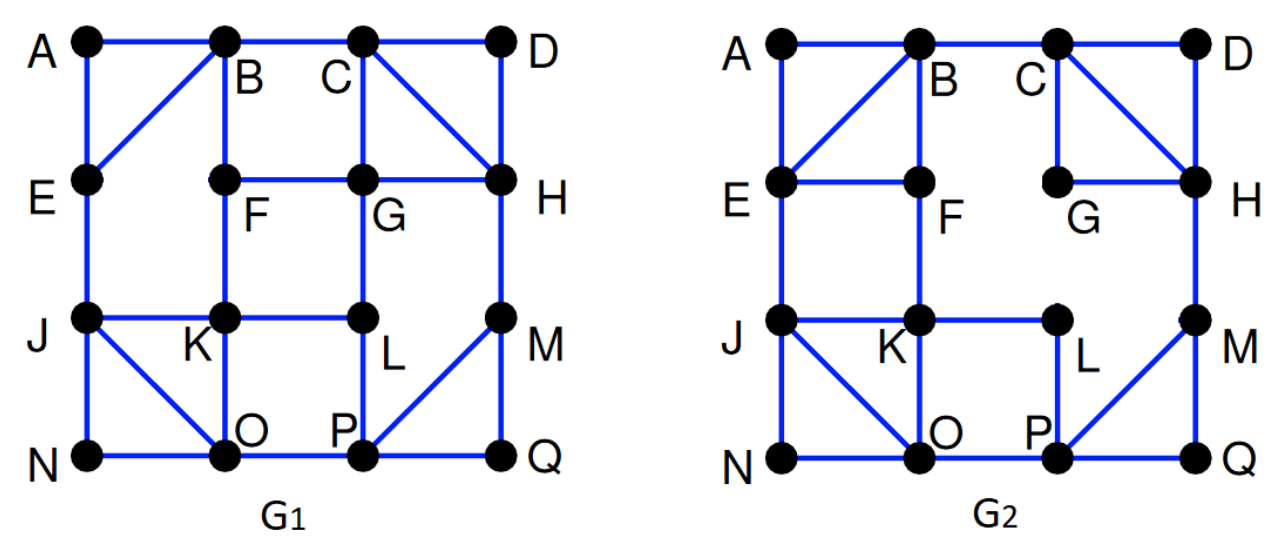
\includegraphics[scale = 0.6]{graphs.png}
        \end{center}

        \answer 

        From the lectures we know that 

        \begin{theorem}
            A graph G contains an Euler circuit if and only if the degree of
            each vertex is even.
        \end{theorem}

        \textit{\textbf{\centerline{A condition for an Euler path to exist}}}


        \begin{theorem}
            A graph G contains an Euler path if and only if there are $2$ odd degree vertices.

            \begin{proof} 

                $\Rightarrow$ Suppose that $G$ does indeed contain an euler path $P$ then for any $\text{vertex} \in P$. $P$ must enter and leave $v$ the same amount of times (i.e. an even number of times) \textit{except} when $v$ is the final or starting vertex of $P$. 

                This is because if a middle vertex in a path was odd then you would get, so there would be no way to leave.

                When the starting and final vertices are distinct then they must be odd so there are exactly $2$ of them.

                $\Leftarrow$ Conversely, assume $\exists x,y \in V(G)$ which both have an odd degree. Add an edge between these vertices $\{x,y\}$ - now in this graph there are no more odd degree vertices \textit{and} $G$ by Theorem 5 above, we know that this graph
                must contain an Euler Circuit $C$ since there only exists even degree vertices.

                Now remove the edge $\{x,y\}$ from the Euler Circuit $C$, we now have an Euler Path where $x,y$ are both of odd degree and they are the initial and starting vertices. 
            \end{proof}
        \end{theorem}

        \pagebreak


        If we look at $G_1$ we can see that vertices $E,F,L,M$ all have an odd degree (specifically a degree of $3$) so by Theorem 6, we can conclude that $G_1$ does \textit{not} have an Euler path.
        

        Consider $G_2$, $G_2$ has a euler path because there are only $2$ vertices which have an odd degree (namely $F,M$ each with degree $3$) with the other vertices having an even degree. 

        We shall aim to find this euler path which beings at $F$ and ends at $M$.

        By inspection we get (I represents 2 ways of representing the path, the first is traversing through the edges and the last one is going through the vertices):

        $$ P = (F, K) \to (K, O) \to (O, P) \to (P, L) \to (L, K) \to (K, J) \to (J,N) \to  (N,O) \to (O,J) \to (J,E)$$
        $$ P_{continue} = (J,E) \to (E,B) \to (B,A) \to (A,E) \to (E,F) \to (F,B) \to (B,C) \to (C,D) \to (D,H) \to (C,G)$$
        $$ P_{continue} = (C,G) \to (G,H) \to (H,M) \to (M,P) \to (P,Q) \to (Q,M) $$

        $P = F \to K \to O \to P \to L \to K \to J \to N \to O \to J \to E \to B \to A \to E \to F \to B \to C \to D \to H \to C \to G \to H \to M \to P \to Q \to M$

        $\boxed{P = F,K,O,P,L,K,J,N,O,J,E,B,A,E,F,B,C,D,H,C,G,H,M,P,Q,M}$

    \end{homeworkProblem}

    \pagebreak








    \end{document}